\def\linkdethi{} %Đường link cần dẫn tới
\anmaQR
%%%%%%%%%%%%%%%%%%%%%%%%
\def\toanlop{12}
\def\thoigian{90}
\def\namhoc{2025 - 2026}
\begin{dethi}
	{Bộ GD\&ĐT}
	{VTED ft KING EDU}
	{TDMT02}
	{Đề thi thử THPTQG 2026}
\end{dethi}
\caulc
\Opensolutionfile{ans}[ans/ansTN-Dung]
%%%=============EX_1=============%%%
\begin{ex}[Đề chính thức 2025]%[1H4N3-2]%[TDMT02]%[Nguyễn Trí Minh Tuấn]
	\immini[thm]{Cho hình hộp $ABCD.A'B'C'D'$ (xem hình bên). Đường thẳng $AB$ song song với mặt phẳng nào dưới đây?
		\choice
		{$(CC'A'A)$}
		{$(ABCD)$}
		{\True $(A'B'C'D')$}
		{$(DD'A'A)$}
	}{
		\begin{tikzpicture}[declare function={a=2; b=0.45*a; h=0.65*a;}]
			\path (0:0) coordinate (A)
			(220:b) coordinate (B)
			($(B)+(a,0)$) coordinate (C)
			(a,0) coordinate (D)
			\foreach \x in {A,B,C,D}{(\x)++(90:h) coordinate (\x1)};
			\draw[dashed] (A1)--(A)--(B) (A)--(D);
			\draw (B1)--(A1)--(D1)--(C1) (D1)--(D)--(C) (B)--(C)--(C1)--(B1)--cycle;
			\foreach \x/\goc/\t in {A/45/A,B/-90/B,C/-90/C,D/0/D,A1/90/A',B1/90/B',C1/90/C',D1/90/D'}
			\fill (\x) circle (1pt) node[shift={(\goc:7pt)},font=\scriptsize]{$\t$};
		\end{tikzpicture}
		}
	\loigiai{
		Ta có $\heva{&AB \parallel A'B'\\ &A'B' \subset \left(A'B'C'D'\right)}$ nên $AB \parallel \left(A'B'C'D'\right)$.
	}
\end{ex}
%%%=============================%%%

%%%=============EX_2=============%%%
\begin{ex}[Đề chính thức 2025]%[1D2N2-3]%[TDMT02]%[Trần Văn Thiện]
	Cho cấp số cộng $(u_{n})$ có $u_{1} = 4$ và công sai $d = -3$. Giá trị của $u_{5}$ bằng
	\choice
	{$16$}
	{$-11$}
	{\True $-8$}
	{$19$}
	\loigiai{
		Ta có $u_{5} = u_{1} + 4\cdot d = 4 + 4\cdot(-3) = -8$.
	}
\end{ex}
%%%=============================%%%

%%%=============EX_3=============%%%
\begin{ex}[Đề chính thức 2025]%[1D1N5-3]%[TDMTD02]%[Phạm Hải Dương]
	Tập nghiệm của phương trình $\sin x = 0$ là
	\choice
	{$S = \left\{\dfrac{\pi}{2} + k\pi \mid k \in \mathbb{Z}\right\}$}
	{$S = \left\{k2\pi \mid k \in \mathbb{Z}\right\}$}
	{$S = \left\{\dfrac{\pi}{2} + k2\pi \mid k \in \mathbb{Z}\right\}$}
	{\True $S = \{k\pi \mid k \in \mathbb{Z}\}$}
	\loigiai{
		Ta có $\sin x = 0\Leftrightarrow x=k\pi,\, k \in \mathbb{Z}$.
	}
\end{ex}
%%%=============================%%%

%%%=============EX_4=============%%%
\begin{ex}[Đề chính thức 2025]%[1D6N4-2]%[TDMT02]%[Văn Minh Thoại]
	Nghiệm của phương trình $\log_{3}(2x - 1) = 2$ là
	\choice
	{$x = \dfrac{7}{2}$}
	{$x = \dfrac{5}{2}$}
	{\True $x = 5$}
	{$x = 4$}
	\loigiai{
		Tập xác định $\mathscr{D} = \left[\dfrac{1}{2};+ \infty\right)$.\\ Ta có
		\begin{eqnarray*}
			&&\log_{3}(2x - 1) = 2\\
			&\Leftrightarrow& 2x- 1=3^{2}\\
			&\Leftrightarrow& x = 5.
		\end{eqnarray*}
		Vậy nghiệm của phương trình là $x=5$.
	}
\end{ex}
%%%=============================%%%

%%%=============EX_5=============%%%
\begin{ex}[Đề chính thức 2025]%[1H8N7-2]%[TDMT02]%[Lê Phúc]
	\immini[thm]{Cho hình chóp $S. ABC$ có cạnh bên $SA$ vuông góc với đáy $(ABC)$, tam giác $ABC$ vuông tại $A$ và $SA = 3$, $AB = 4$, $AC = 5$. Thể tích của khối chóp $S.ABC$ bằng
		\choice
		{$20$}
		{$30$}
		{\True $10$}
		{$60$}}
	{
		\begin{tikzpicture}[declare function={a=2; b=0.45*a; h=0.65*a;}]
			\path (0,0) coordinate (A)
			(a,0) coordinate (C)
			(-45:b) coordinate (B)
			($(A)+(0,h)$) coordinate (S);
			\foreach \x/\y/\z in {B/A/S,C/A/S,B/A/C}{
				\path pic[draw,angle radius=5pt]{right angle=\x--\y--\z};
			}
			\draw[dashed] (A)--(C);
			\draw (S)--(B)
			(S)--(A)--(B)--(C)--cycle;
			\foreach \x/\goc in {S/90,A/190,B/-90,C/0}
			\fill (\x) node[shift={(\goc:7pt)},font=\scriptsize]{$\x$} circle (1pt);
		\end{tikzpicture}
	}
	\loigiai{
		Thể tích của khối chóp là
		\[V = \dfrac{1}{3} \cdot S_{ABC} \cdot SA=\dfrac{1}{3}\cdot\dfrac{1}{2}\cdot AB\cdot AC\cdot SA = \dfrac{1}{3} \cdot \dfrac{1}{2}\cdot 4\cdot 5 \cdot3 = 10.\]
	}
\end{ex}
%%%=============================%%%

%%%=============EX_6=============%%%
\begin{ex}%[2D1H1-1]%[TDMT02]%[Vũ Hồng Toàn]
	Hàm số $y = x^3 - 6x^2 + 1$ nghịch biến trên khoảng
	\choice
	{$\left(-2;2\right)$}
	{$\left(-\infty;0\right)$}
	{$\left(4;+\infty\right)$}
	{\True $\left(0;4\right)$}
	\loigiai{
		Tập xác định $\mathscr{D}=\mathbb{R}$.\\
		Ta có $y' = 3x^2 - 12x = 3x\left(x - 4\right) = 0 \Leftrightarrow \hoac{&x = 0\\&x = 4.}$\\
		Bảng biến thiên
		\begin{center}
			
\begin{tikzpicture}
				\tkzTabInit[nocadre=false, lgt=1.2, espcl=3, deltacl=0.5]
				{$x$/0.7,$y'$/0.7, $y$/2}
				{$-\infty$,$0$,$4$,$+\infty$}
				\tkzTabLine{,+,0,-,0,+,}
				\tkzTabVar{-/$-\infty$, +/$1$, -/$-31$, +/$+\infty$}
			\end{tikzpicture}
		\end{center}
		Dựa vào bảng biến thiên ta thấy hàm số nghịch biến trên khoảng $\left(0;4\right)$.
	}
\end{ex}
%%%=============================%%%

%%%=============EX_7=============%%%
\begin{ex}%[1D3H2-4]%[TDMT02]%[Chu Ha]
	Giới hạn $\lim\limits_{x\to+\infty}\left(\sqrt{x^2 + 2x} - 3x\right)$ bằng
	\choice
	{$+\infty$}
	{$\dfrac{1}{2}$}
	{\True $-\infty$}
	{$1$}
	\loigiai{
		Ta có
		$\lim\limits_{x\to+\infty}\left(\sqrt{x^2 + 2x} - 3x\right)
		=\lim\limits_{x\to+\infty}x\left(\sqrt{1 + \dfrac{2}{x}} - 3\right)
		=-\infty$ (vì $\lim\limits_{x\to+\infty}=+\infty$ và $\lim\limits_{x\to+\infty}\left(\sqrt{1+\dfrac{2}{x}}-3\right)=-2<0$).
	}
\end{ex}
%%%=============================%%%

%%%=============EX_8=============%%%
\begin{ex}%[2D1N2-2]%[TDMT02]%[Nguyễn Sơn Thành]
	Cho hàm số $f(x)$ có bảng biến thiên như hình vẽ bên dưới. Hỏi hàm số $f(x)$ có tất cả bao nhiêu điểm cực trị?
	\begin{center}
		\begin{tikzpicture}[font=\normalsize,t style/.style={style=solid}]
			\tkzTabInit[nocadre=false, lgt=1.2, espcl=2.5, deltacl=0.5]
			{$x$/0.75, $f(x)$/3}
			{$-\infty$, $-3$, $0$, $2$, $+\infty$}
			\path
			($(N12)!0.1!(N11)$) node (A1){$ -\infty $}
			($(N22)!0.8!(N21)$) node (A2){$ 4 $}
			($(N32)!0.25!(N31)$) node (A3){$ -2 $}
			($(N42)!0.65!(N41)$) node (A4){$ 3 $}
			($(N52)!0.1!(N51)$) node (A5){$ -\infty $};
			\foreach \x/\y in {A1/A2, A2/A3, A3/A4, A4/A5}{
				\draw[-stealth] (\x)--(\y);
			}
		\end{tikzpicture}
	\end{center}
	\choice
	{\True $3$}
	{$2$}
	{$1$}
	{$0$}
	\loigiai{
		Dựa vào bảng biến thiên ta thấy hàm số có $3$ điểm cực trị.	
	}
\end{ex}
%%%=============================%%%

%%%=============EX_9=============%%%
\begin{ex}%[2D1N2-1]%[Đỗ Đường Hiếu]
	Hỏi hàm số nào dưới đây \textbf{không} có cực trị?
	\choice
	{$y = x^2$}
	{\True $y = \mathrm{e}^{x}$}
	{$y = x^3 - 2\,026x$}
	{$y = \sin x$}
	\loigiai{
		Xét $y = \mathrm{e}^{x}$ ta có $y' = \mathrm{e}^{x} > 0$, $\forall x \in \mathbb{R}$.\\
		Do đó hàm số $y = \mathrm{e}^{x}$ không có cực trị.
	}
\end{ex}
%%%=============================%%%

%%%=============EX_10=============%%%
\begin{ex}%[2D1H3-1]%[TDMT02]%[Huỳnh Quốc Đạt]
	Giá trị nhỏ nhất của hàm số $y = x^4 - 4x$ trên đoạn $\left[0;2\right]$ là
	\choice
	{$\min\limits_{\left[0;2\right]} y = 1$}
	{$\min\limits_{\left[0;2\right]} y = 0$}
	{$\min\limits_{\left[0;2\right]} y = -5$}
	{\True $\min\limits_{\left[0;2\right]} y = -3$}
	\loigiai{
		Ta có $y' = 0 \Leftrightarrow 4x^3-4 = 0\Leftrightarrow x=1 \in \left[0;2\right]$\\
		Khi đó $y(0) = 0$, $y(2) = 8$, $y(1) = -3$.\\
		Vậy $\min\limits_{\left[0;2\right]} y = y(-1) = -3$.
	}
\end{ex}
%%%=============================%%%

%%%=============EX_11=============%%%
\begin{ex}%[1D9N1-1]%[TDMTD02]%[Dương Công Tạo]
	Cho hai biến cố $A$, $B$ của một phép thử $T$ được gọi là xung khắc nếu
	\choice
	{$\mathrm{P}(AB) = \mathrm{P}(A)\cdot\mathrm{P}(B)$}
	{\True $\mathrm{P}(AB) = 0$}
	{$\mathrm{P}(A\cup B) = \mathrm{P}(A)\cdot\mathrm{P}(B)$}	
	{$\mathrm{P}(AB) = \mathrm{P}(A) + \mathrm{P}(B)$}
	\loigiai{
		Hai biến cố $A$, $B$ của một phép thử $T$ được gọi là xung khắc nếu $\mathrm{P}(AB) = 0$ (vì $(A \cap B = \varnothing)$).
	}
\end{ex}
%%%=============================%%%

%%%=============EX_12=============%%%
\begin{ex}%[2D1H2-1]
	Trong mặt phẳng tọa độ, gọi $A$ và $B$ là hai điểm cực trị của đồ thị hàm số $y=\dfrac{x^2-4x+5}{x-1}$. Phương trình đường thẳng $AB$ có phương trình là
	\choice
	{\True $y=2x-4$}
	{$y=x-4$}
	{$y=x-3$}
	{$y=2x-1$}
	\loigiai
	{
		Phương trình đường thẳng đi qua hai điểm cực trị là $y=\dfrac{(x^2-4x+5)'}{(x-1)'}=2x-4$.
	}
\end{ex}
%%%=============================%%%
\Closesolutionfile{ans}

\cauds
\Opensolutionfile{ans}[ans/ansTN-DungSai]
%%%=============EX_13=============%%%
\begin{ex}[Đề chính thức 2025]%[2D1H3-1]%[Duong Xuan Loi]
	Cho hàm số $f(x) = x^3 - 12x - 8$.
	\choiceTF[t]
	{\True $f'(x) = 3x^2 - 12$}
	{Phương trình $f'(x) = 0$ có tập nghiệm là $S = \{2\}$}
	{$f(2) = 24$}
	{Giá trị lớn nhất của hàm số $f(x)$ trên đoạn $\left[-3;3\right]$ bằng $24$}
	\loigiai{
		\begin{itemchoice}
			\itemch $f'(x) = 3x^2 - 12$.
			\itemch $f'(x) = 0 \Leftrightarrow x^2 = 4 \Leftrightarrow x = \pm 2 \Rightarrow S = \{2;-2\}$.
			\itemch $f(2) = 2^3 - 12 \cdot 2 - 8 = -24$.
			\itemch Ta có $f(-3) = 1$; $f(3) = -17$; $f(2) = -24$; $f(-2) = 8$.\\
			Vậy $\max\limits_{\left[-3;3\right]} f(x) = 8$.
		\end{itemchoice}
	}
\end{ex}
%%%=============================%%%

%%%=============EX_14=============%%%
\begin{ex}%[2D1V3-6]
	Một cây đậu Hà Lan khi mới trồng cao $4$ cm. Gọi $h(t)$ là độ cao tính bằng centimet của cây đậu này ở thời điểm $t$ kể từ khi được trồng, với $t$ được tính theo tuần. Khảo sát cho thấy chiều cao này được mô hình hóa bởi hàm số $h(t) = -0{,}005t^4 + 0{,}1t^3 + c$ (cm).
	\choiceTF[t]
	{\True $c = 4$}
	{\True Tốc độ tăng chiều cao của cây đậu này ở tuần thứ hai là $1{,}04$ cm/tuần}
	{\True Cây đậu này có tộc độ tăng chiều cao lớn nhất bằng $10$ cm/tuần}
	{Chiều cao lớn nhất của cây đậu này là $96$ cm}
	\loigiai{
		\begin{itemchoice}
			\itemch $h(0) = 4 \Leftrightarrow c = 4$.
			\itemch $h'(t) = -0{,}02t^3 + 0{,}3t^2$ (cm/tuần); $h'(2) = 1{,}04$ (cm/tuần).
			\itemch $\left[h'(t)\right]' = h''(t) = -0{,}06t^2 + 0{,}6t = 0 \Leftrightarrow \hoac{&t = 0\\&t = 10.}$\\
			\begin{center}
				
\begin{tikzpicture}
					\tkzTabInit[lgt=1.2,espcl=3,nocadre=false]
					{$t$/0.7,$h''(t)$/0.7, $h'(t)$/2}
					{$0$,$10$,$+\infty$}
					\tkzTabLine{0,+,0,-,}
					\tkzTabVar{-/, +/$\max$, -/}
				\end{tikzpicture}
			\end{center}
			Vậy $\max\limits_{\left[0;+\infty\right)} h'(t) = h'(10) = 10$ (cm/tuần).
			\itemch $h'(t) = 0 \Leftrightarrow \hoac{&t = 0\\&t = 15.}$
			\begin{center}
				
\begin{tikzpicture}
					\tkzTabInit[lgt=1.2,espcl=3,nocadre=false]
					{$t$/0.7,$h'(t)$/0.7, $h(t)$/2}
					{$0$,$15$,$+\infty$}
					\tkzTabLine{,+,0,-,}
					\tkzTabVar{-/$4$, +/$\max$, -/}
				\end{tikzpicture}
			\end{center}
			Vậy $\max\limits_{\left[0;+\infty\right)} h(t) = h(15) = 88{,}375$ (cm).
		\end{itemchoice}
	}
\end{ex}
%%%=============================%%%

%%%=============EX_15=============%%%
\begin{ex}%[1H8V6-2]%[TDMT02]%[Lê Hồ Quang Minh]
	\immini[thm]{Cho hình lăng trụ đều $ABC.A'B'C'$ có các cạnh $AB = 6$, $AA' = 8$.
		\choiceTF[t]
		{\True Thể tích của khối lăng trụ đều $ABC.A'B'C'$ bằng $72\sqrt{3}$}
		{$\mathrm{d}(AA',BC) = 2\sqrt{3}$}
		{Số đo góc nhị diện $\left[A,B'C',A'\right]$ bằng $60^{\circ}$ (\textit{làm tròn kết quả đến hàng đơn vị})}
		{Góc giữa hai mặt phẳng $\left(AB'C'\right)$, $\left(B'AC\right)$ bằng $48^{\circ}$ (\textit{làm tròn kết quả đến hàng đơn vị})}
		}{
			\begin{tikzpicture}[
			declare function={a=4; b=0.55*a; h=0.9*a;},
			line cap=round,line join=round,font=\footnotesize,>=stealth,scale=1
			]
			\path (0:0) coordinate (A')
			(-30:b) coordinate (B')
			(a,0) coordinate (C');
			\path (A') ++(90:h) coordinate (A)
			(B') ++(90:h) coordinate (B)
			(C') ++(90:h) coordinate (C);
			\path ($(B)!.5!(C)$) coordinate (M)
			($(B')!.5!(C')$) coordinate (N)
			(intersection of A--C' and A'--C) coordinate (I);
			\draw (A) -- (B) -- (C) -- cycle; 
			\draw (A) -- (A') -- (B') -- (C') -- (C); 
			\draw (B) -- (B');
			\draw[dashed] (A') -- (C') (C) -- (A') (A)--(N)--(A') (A)--(C');
			\draw (M)--(A)--(B')--(C);
			\pic[draw,angle radius=3mm] {right angle = A--M--B};
			\foreach \i/\r in {A/145,B/90,C/45,M/90,A'/-135,B'/-90,C'/-45,N/-15,I/-90}{
				\filldraw[black] (\i) circle (1pt);
				\node at ($(\i) + (\r:3mm)$) {$\i$};
			}
		\end{tikzpicture}}
	\loigiai{
		\begin{itemchoice}
			\itemch Ta có $S_{\text{đáy}} = \dfrac{6^2\cdot \sqrt{3}}{4} = 9\sqrt{3}$ và $h = AA' = 8$.\\
			Vậy thể tích khối lăng trụ là $V = S_{\text{đáy}} \cdot h = 9\sqrt{3} \cdot 8 = 72\sqrt{3}$.
			\itemch Gọi $M$ là trung điểm của $BC$.\\
			Dễ thấy $AM \perp \left(BB'C'C\right)$ và $AA' \parallel \left(BB'C'C\right)$.\\
			Khi đó $\mathrm{d}(AA',BC) = \mathrm{d}(AA',(BCC'B')) = \mathrm{d}(A,(BCC'B')) = AM = \dfrac{6\sqrt{3}}{2} = 3\sqrt{3}$.
			\itemch Gọi $N$ là trung điểm của $B'C'$.\\
			Ta có $A'N\perp BC$, $AN\perp BC$.\\
			Khi đó $\text{sđ}\left[A, B'C', A'\right] = \widehat{ANA'}$.\\
			Ta có $\tan \widehat{ANA'} = \dfrac{AA'}{A'N} = \dfrac{8}{\tfrac{6\sqrt{3}}{2}} = \dfrac{8}{3\sqrt{3}}$.\\
			Vậy $\widehat{ANA'} = \arctan \dfrac{8}{3\sqrt{3}} \approx 57^{\circ}$.
			\itemch Ta có $A'C = AB' = B'C = 10$.\\ 
			Đặt $A'N= 3\sqrt{3}$.\\
			Ta có
			\[\mathrm{d}\left(C,(AB'C')\right) = \dfrac{CI}{AI}\cdot\mathrm{d}\left(A',(AB'C')\right) = \mathrm{d}\left(A',(AB'C')\right) = \dfrac{AA'\cdot A'N}{\sqrt{AA'^2 + A'N^2}} = \dfrac{8\cdot3\sqrt{3}}{\sqrt{8^2 + \left(3\sqrt{3}\right)^2}} = \dfrac{24\sqrt{273}}{91}.\]
			Xét hình vẽ sau
			\begin{center}
			\begin{tikzpicture}[
				declare function={a=5; b=2; goc=-150;},
				line cap=round, line join=round, font=\footnotesize, >=stealth, scale=1
				]
				\path
				(0,0) coordinate (A)
				(a,0) coordinate (B)
				(goc:b) coordinate (D)
				($(D)+(B)$) coordinate (J)
				($(J)!.7!-60:(D)$) coordinate (E)
				($(B)!.7!-60:(A)$) coordinate (F)
				(intersection of A--B and E--J) coordinate (G)
				($(B)!0.5!(J)$) coordinate (H)
				($(E)!0.5!(F)$) coordinate (I)
				($(H)!3/4!(I)$) coordinate (C)
				($(A)!0.5!(D)$) coordinate (K)
				($(H)!(I)!(K)$) coordinate (T)
				(intersection of E--J and T--H) coordinate (M)
				(intersection of C--T and E--J) coordinate (N);
				\draw (A) -- (D) -- (J) -- (B)
				(J) -- (E) -- (F) -- (B)
				(A) -- (G)
				(C) -- (H)
				(T) -- (M)
				(T) -- (N);
				\draw[dashed] (G) -- (B)
				(H) -- (M)
				(N) -- (C);
				\pic[draw, angle radius=7mm, angle eccentricity=1.4, "$CAB'$"] {angle = E--F--B};
				\pic[draw, angle radius=10mm, angle eccentricity=1., "$AB'C'$"] {angle = J--D--A};
				\pic[draw, angle radius=5mm, angle eccentricity=1.5, "$\varphi$"] {angle = C--H--T};
				\pic[draw, angle radius=2mm] {right angle = C--T--H};
				\foreach \i/\r in {H/0, C/180, T/-90}{
					\filldraw[black] (\i) circle (1pt);
					\node at ($(\i) + (\r:3mm)$) {$\i$};
				}
			\end{tikzpicture}			
			\begin{tikzpicture}[
				line cap=round, line join=round, font=\footnotesize, >=stealth, scale=1
				]
				\path
				(0,0) coordinate (A)
				(4,0) coordinate (C)
				(2,4) coordinate (B')
				($(A)!(B')!(C)$) coordinate (h)
				($(B')!(C)!(A)$) coordinate (H);
				\draw (A) -- (B') node[midway, left] {$10$}
				-- (C) node[midway, right] {$10$}
				-- cycle;
				\draw (B') -- (h);
				\draw (C) -- (H);
				\node[below] at ($(A)!0.5!(h)$) {$3$};
				\node[below] at ($(h)!0.5!(C)$) {$3$};
				\pic[draw, angle radius=2.5mm] {right angle = A--H--C};
				\pic[draw, angle radius=2.5mm] {right angle = C--h--B'};
				\pic[draw, angle radius=5mm, angle eccentricity=1.4, "$\alpha$"] {angle = C--A--B'};
				\foreach \i/\r in {A/-135, B'/90, C/-45, H/180}{
					\filldraw[black] (\i) circle (1pt);
					\node at ($(\i) + (\r:3mm)$) {$\i$};
				}
			\end{tikzpicture}
			\end{center}
			Ta có $\cos \alpha = \dfrac{3}{10} \Rightarrow \sin \alpha = \dfrac{\sqrt{91}}{10} \Rightarrow CH = \mathrm{d}(C,AB') = AC \sin \alpha = 6 \cdot \dfrac{\sqrt{91}}{10} = \dfrac{3\sqrt{91}}{5}$.\\
			Suy ra
			$\sin\left((AB'C'),(B'AC)\right) = \dfrac{\mathrm{d}\left(C,(AB'C')\right)}{\mathrm{d}\left(C,AB'\right)} = \dfrac{40\sqrt{3}}{91}$.\\
			Vậy góc cần tìm là $\arcsin \dfrac{40\sqrt{3}}{91} \approx 49{,}58^{\circ}$.
		\end{itemchoice}
	}
\end{ex}
%%%=============================%%%

%%%=============EX_16=============%%%
\begin{ex}%[2D1C2-6]%[TDMT02]%[Lương Pho]
	Cho hàm số $f(x) = \dfrac{x^2 - bx + c}{x - 1}$ có đồ thị $(C)$, với $b$ và $c$ là các số thực.
	\choiceTF[t]
	{Khi $b = 4$, $c = 7$ thì hàm số đồng biến trên từng khoảng xác định}
	{\True Khi $b = 4$, $c = 7$ thì hàm số có hai điểm cực trị}
	{\True Khi $b = 4$, $c = 7$ thì đường thẳng đi qua hai điểm cực trị có phương trình là $y = 2x - 4$}
	{\True Tiến hành gieo một con xúc xắc cân đối đồng chất hai lần liên tiếp, số chấm thu được ở lần một đặt bằng $b$ và lần hai đặt bằng $c$. Xác suất để hàm số $f(x) = \dfrac{x^2 - bx + c}{x - 1}$ có hai điểm cực trị là $0{,}58$ (\textit{làm tròn kết quả đến hàng phần trăm})}
	\loigiai{
		Với $b = 4$, $c = 7$ thì $f(x) = \dfrac{x^2 - 4x + 7}{x - 1}$ và $f'(x) = \dfrac{x^2 - 2x - 3}{(x - 1)^2} = 0 \Leftrightarrow \hoac{&x = -1\\& x = 3.}$\\
		Bảng biến thiên
		\begin{center}
			
\begin{tikzpicture}
				\tkzTabInit[nocadre=false,lgt=1.2,espcl=2.5, deltacl=0.5]
				{$x$/0.7,$f'(x)$/0.7, $f(x)$/2}
				{$-\infty$, $-1$, $1$, $3$, $+\infty$}
				\tkzTabLine{,+,0,-,d,-,0,+,}
				\tkzTabVar{-/$-\infty$, +/$-6$, -D+/$-\infty$/$+\infty$, -/$2$, +/$+\infty$}
			\end{tikzpicture}
		\end{center}
		\begin{itemchoice}
			\itemch Khi $b = 4$, $c = 7$ thì hàm số đồng biến trên $(-\infty;-1)$ và $(3;+\infty)$.
			\itemch Khi $b = 4$, $c = 7$ thì hàm số có hai điểm cực trị.
			\itemch Với $b = 4$, $c = 7$ thì $f(x) = \dfrac{x^2 - 4x + 7}{x - 1}$.\\
			Đường thẳng đi qua hai điểm cực trị của đồ thị hàm số $y = \dfrac{(x^2 - 4x + 7)'}{(x-1)'} = 2x - 4$.
			\itemch Số phần tử không gian mẫu là $n(\Omega) = 6^2 = 36$.\\
			Điều kiện đề hàm số $f(x)$ có hai điểm cực trị khi và chỉ khi $f'(x)=\dfrac{x^2-2x+(b-c)}{(x-1)^2}=0$ có hai nghiệm phân biệt.\\
			Khi đó $\Delta '=1^2-(b-c)>0\Leftrightarrow 1+c>b$.\\
			Do $b$, $c\in \{1;2;3;4;5;6\}$ nên
			\begin{itemize}
				\item Với $c=1$, ta chọn được $b=1$. Có $1$ bộ $(b;c)$.
				\item Với $c=2$, ta chọn được $b=1;2$. Có $2$ bộ $(b;c)$.
				\item Với $c=3$, ta chọn được $b=1;2;3$. Có $3$ bộ $(b;c)$.
				\item Với $c=4$, ta chọn được $b=1;2;3;4$. Có $4$ bộ $(b;c)$.
				\item Với $c=5$, ta chọn được $b=1;2;3;4;5$. Có $5$ bộ $(b;c)$.
				\item Với $c=6$, ta chọn được $b=1;2;3;4;5;6$. Có $6$ bộ $(b;c)$.
			\end{itemize}
			Số kết quả thuận lợi là $n(A)=1+2+3+4+5+6=21$.\\
			Vậy xác suất lcần tìm là $\mathrm{P}(A) = \dfrac{21}{36} \approx 0{,}58$.
		\end{itemchoice}
	}
\end{ex}
%%%=============================%%%
\Closesolutionfile{ans}

\caukq 
\Opensolutionfile{ans}[ans/ansTN-DienKhuyet]
%%%=============EX_17=============%%%
\begin{ex}%[2D1H2-2]%[TDMT02]%[Võ Hiệp]
	Cho hàm số $f(x)$ có bảng biến thiên đạo hàm $f'(x)$ như hình vẽ bên dưới. Hàm số $f(x)$ có bao nhiêu điểm cực trị?
	\begin{center}
		
\begin{tikzpicture}
			\tkzTabInit[lgt=1.2,espcl=2.5,nocadre=false]
			{$x$/0.7,$f'(x)$/2}
			{$-\infty$, $-3$, $2$, $+\infty$}
			\tkzTabVar{-/$-\infty$, +/$3$, -/$-3$, +/$+\infty$}
		\end{tikzpicture}
	\end{center}
	\par
	\shortans[oly]{3}
	\loigiai{
		\begin{center}
			\begin{tikzpicture}
				\tkzTabInit[nocadre=false,lgt=1.2,espcl=2.5,deltacl=0.6]
				{$x$/0.7,$f'(x)$/2.2}
				{$-\infty$, $-3$, $2$, $+\infty$}
				\tkzTabVar{-/$-\infty$, +/$3$, -/$-3$, +/$+\infty$}
				\draw ($(T11)!.5!(T12)$)--($(T21)!.5!(T22)$)node[above,pos=.1]{$f'(x)=0$};
			\end{tikzpicture}
		\end{center}
		Dựa vào bảng biến thiên của hàm số $f'(x)$, ta có\\
		Phương trình $f'(x)=0 \Leftrightarrow \hoac{&x=a& (a<-3)\\&x=b &(-3<b<2)\\&x=c&(c>2).}$\\
		Do đó $f'(x)$ đối dấu tại các điểm $x=a$, $x=b$, $x=c$.\\
		Suy ra hàm số $f(x)$ có $3$ điểm cực trị.
	}
\end{ex}
%%%=============================%%%

%%%=============EX_18=============%%%
\begin{ex}%[1H8V7-6]%[TDMT02]%[Nguyễn Đức Tuấn Anh]
	Cho hình chóp cụt đều $ABCD. A'B'C'D'$ có hai cạnh đáy là $AB = 4$, $A'B' = 6$ và cạnh bên $AA' = 4$. Tính thể tích khối chóp cụt $ABCD. A'B'C'D'$ (\textit{không làm tròn các phép tính trung gian, chỉ làm tròn kết quả cuối cùng đến hàng phần mười}).
	\par
	\shortans[oly]{94{,}8}
	\loigiai{
		\begin{center}
			\begin{tikzpicture}[
				declare function={a=5; b=2.5; h=6; goc=-135;},
				line cap=round, line join=round, font=\footnotesize, >=stealth, scale=1
				]
				\path
				(0,0) coordinate (B')
				(a,0) coordinate (C')
				(goc:b) coordinate (A')
				($(A')+(C')$) coordinate (D') 
				($(B')!.5!(D')$) coordinate (O');
				\path
				($(O') + (0,h)$) coordinate (S)
				($(A')!.4!(S)$) coordinate (A)
				($(B')!.4!(S)$) coordinate (B)
				($(C')!.4!(S)$) coordinate (C)
				($(D')!.4!(S)$) coordinate (D)
				($(B)!.5!(D)$) coordinate (O);
				\path
				($(A)+(0,-1)$) coordinate (Ah)
				($(C)+(0,-1)$) coordinate (Ch)
				(intersection of A--Ah and A'--C') coordinate (H)
				(intersection of C--Ch and A'--C') coordinate (K);
				\draw[dashed] (B) -- (B')
				(A') -- (B') -- (C')
				(O) -- (O')
				(B') -- (D')
				(A') -- (C')
				(A) -- (H)
				(C) -- (K);
				\draw (A') -- (D') -- (C') -- (C) -- (D) -- (A) -- (B) -- (C)
				(D') -- (D)
				(A') -- (A)
				(B) -- (D)
				(A) -- (C);
				\pic[draw, angle radius=2.5mm] {right angle= O--O'--A'};
				\pic[draw, angle radius=2.5mm] {right angle= A--O--O'};
				\pic[draw, angle radius=2.5mm] {right angle= A--H--A'};
				\pic[draw, angle radius=2.5mm] {right angle= C--K--C'};
				\foreach \i/\r in {B'/-90, C'/0, D'/-60, A'/-180, O'/-95, B/90, C/90, D/90, A/90, O/90, H/-45, K/-90}{
					\filldraw[black] (\i) circle (1pt);
					\node at ($(\i) + (\r:3mm)$) {$\i$};
				}
			\end{tikzpicture}	
		\end{center}
		Do $ABCD$ và $A'B'C'D'$ là hình vuông có cạnh lần lượt là $4$ và $6$ nên $AC=4\sqrt{2}$ và $A'C'=6\sqrt{2}$.\\
		Kẻ $A'H \perp AC$, $C'K \perp AC$.\\
		Khi đó, $A'C'CA$ là hình chữ nhật nên $HK=AC =4\sqrt{2}$.\\
		Do đó $A'H = C'K = \dfrac{A'C' - AC}{2} = \sqrt{2}$.\\
		Xét $\triangle AA'H$ vuông tại $H$, ta có $AH = \sqrt{4^2 - \left(\sqrt{2}\right)^2} = \sqrt{14}$. \\
		Thể tích của hình chóp cụt đều là
		\[V = \dfrac{S_{ABCD} + S_{A'B'C'D'} + \sqrt{S_{ABCD}\cdot S_{A'B'CD'}}}{3}\cdot SH = \dfrac{4^2 + 6^2 + \sqrt{4^2\cdot 6^2}}{3}\cdot \sqrt{14} \approx 94{,}8 \text{ (đơn vị diện tích)}.\]
	}
\end{ex}
%%%=============================%%%

%%%=============EX_19=============%%%
\begin{ex}%[2D1V3-6]%[TDMT02]%[Bồ Văn Hậu]
	\immini[thm]{Dùng một dây thép dài $150$ cm uốn thành một khung có dạng như hình vẽ. Biết phần dưới là hình chữ nhật và phần trên là nửa đường tròn. Hãy tính giá trị lớn nhất của diện tích của khung theo đơn vị centimet vuông \textit{(làm tròn kết quả đến hàng đơn vị)}.}{\begin{tikzpicture}[line cap=round, line join=round, font=\footnotesize, >=stealth, scale=0.7]
			\draw[blue] (0,0) arc[start angle=0, end angle=180, radius=2cm];
			\draw[red] (0,0) -- (0,-3) -- (-4,-3) -- (-4,0);
			\draw[dashed] (0,0)--(-4,0) (-2,2)--(-2,-3);
	\end{tikzpicture}}
	\par 
	\shortans[oly]{1575}
	\loigiai{
		Gọi $x$ (cm), $y$ (cm) lần lượt là bán kính của nửa đường tròn trên, chiều rộng của hình chữ nhật.\\ Điều kiện $x>0$ và $y>0$.\\
		Xét hình vẽ như sau
		\begin{center}
			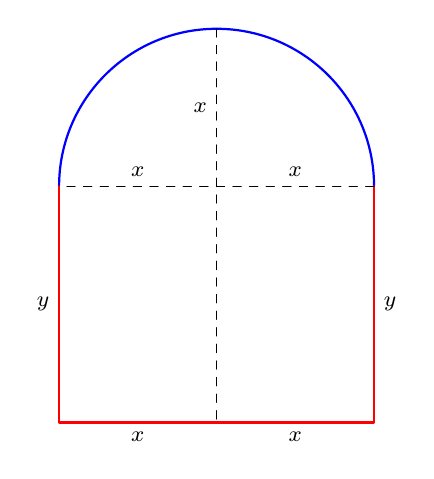
\begin{tikzpicture}[line cap=round, line join=round, font=\footnotesize, >=stealth, scale=1]
				\draw[thick,blue] (0,0) arc[start angle=0, end angle=180, radius=2cm];
				\draw[thick,red] (0,0) -- (0,-3) -- (-4,-3) -- (-4,0);
				\draw[dashed] (0,0) -- (-2,0) node[midway, above] {$x$} -- (-4,0) node[midway, above] {$x$} (-2,2) -- (-2,-3);
				\node[left] at (-2,1) {$x$};
				\node[below] at (-1,-3) {$x$};
				\node[below] at (-3,-3) {$x$};
				\node[right] at (0,-1.5) {$y$};
				\node[left] at (-4,-1.5) {$y$};
			\end{tikzpicture}
		\end{center}
		\noindent
		Dây thép có chiều dài $150$ cm nên ta có \[150 = \pi x + y + 2x + y = (\pi + 2)x + 2y.\]
		Suy ra $y = \dfrac{150 - \left(\pi + 2\right)x}{2}$.\\
		Diện tích của khung
		\[S = 2xy + \dfrac{1}{2}x^2\pi = - \dfrac{\pi + 4}{2}x^2 + 150x = S(x)\,\, \left(\text{cm}^2\right).\]
		Vì đây là hàm số bậc $2$ có hệ số $a < 0$ nên giá trị lớn nhất đạt tại $x = \dfrac{-b}{2a}=\dfrac{150}{\pi + 4}$.\\
		Vậy diện tích lớn nhất của khung là
		\[S_{\max} = S\left(\dfrac{150}{\pi + 4}\right) = 1575{,}27 \approx 1575 \quad \left(\text{cm$^2$}\right).\]
	}
\end{ex}
%%%=============================%%%

%%%=============EX_20=============%%%
\begin{ex}[Đề chính thức 2025]%[TDMT02]%[1H8V5-4]
	Cho hình chóp $S. ABCD$ có đáy $ABCD$ là hình thoi với $\widehat{ABC}=60^{\circ}$ và $AB=2$. Biết rằng hình chiếu vuông góc của $S$ trên mặt phẳng $(ABCD)$ là trọng tâm $H$ của tam giác $ABC$ và $SH=\sqrt{3}$. Khoảng cách giữa hai đường thẳng $AC$ và $SD$ bằng bao nhiêu \textit{(không làm tròn kết quả của các phép tính trung gian, chỉ làm tròn kết quả cuối cùng đến hàng phần trăm)}?
	
	\par
	\shortans[oly]{1,04}
	\loigiai
	{
		\immini
		{
			Gọi $O=AC \cap BD$, kẻ $OF\perp SD$ với $(F \in SD)$ và kẻ $HE \parallel OF$ với $(E \in SD)$.\\
			Ta có $\heva{&AC\perp BD\\&AC\perp SH}\Rightarrow AC\perp (SBD)$.\\
			Suy ra $AC\perp OF$ do đó $\mathrm{d}(AC,SD)=OF$.\\
			Ta có $\dfrac{OF}{HE}=\dfrac{DO}{DH}=\dfrac{3}{4} \Rightarrow OF=\dfrac{3}{4} HE$.\\ Tam giác $ABC$ đều cạnh $2$ $\Rightarrow HB=\dfrac{2}{\sqrt{3}} \Rightarrow HD=2HB=\dfrac{4}{\sqrt{3}}$.\\
			Vậy $OF=\dfrac{3}{4} HE=\dfrac{3}{4}\cdot\dfrac{SH\cdot HD}{\sqrt{SH^2+HD^2}}=\dfrac{3}{4}\cdot\dfrac{\sqrt{3}\cdot\dfrac{4}{\sqrt{3}}}{\sqrt{3+\dfrac{16}{3}}}=\dfrac{3\sqrt{3}}{5} \approx 1{,}04$.
		}
		{
			\begin{tikzpicture}[>=stealth,line join=round,line cap=round,font=\footnotesize,scale=0.75]
				\coordinate (A) at (0,0);
				\coordinate (B) at (-2,-2);
				\coordinate (D) at (5,0);
				\coordinate (C) at ($(B)+(D)-(A)$);
				\coordinate (O) at ($(A)!0.5!(C)$);
				\coordinate (M) at ($(B)!.5!(C)$);
				\coordinate (N) at ($(A)!.5!(B)$);
				\coordinate (H) at ($(A)!2/3!(M)$);
				\coordinate (S) at ($(H)+(0,5)$);
				\coordinate (E) at ($(S)!.45!(D)$);
				\coordinate (F) at ($(S)!.6!(D)$);
				\draw (S)--(B)--(C)--(D)--(S)--(C);
				\draw[dashed] (B)--(A)--(D) (A)--(S)--(H)--(E) (B)--(D) (A)--(C)--(N) (O)--(F) ;
				\foreach \d/\g in {A/180,B/190,C/-50,D/0,S/90,H/-90,E/70,O/-90,F/70}
				\fill[black](\d) circle (1pt)+(\g:.3)node{$\d$};
				\foreach\x/\y/\z in{S/H/D, D/E/H, D/F/O}\pic[draw,angle radius=6]{right angle=\x--\y--\z};
			\end{tikzpicture}
		}
	}
\end{ex}
%%%=============================%%%

%%%=============EX_21=============%%%
\begin{ex}[Đề chính thức 2025]%[Nguyễn Văn Sang]%[TDM-KSCL-DE2]%[0D8C2-5]
	Tiến hành xếp $7$ cuốn sách khác nhau vào một giá sách có $4$ ngăn theo hàng ngang sao cho mỗi ngăn được ít nhất một cuốn và có ít nhất một ngăn có từ $3$ cuốn trở lên. Hai cách xếp được gọi là giống nhau nếu như thỏa mãn đồng thời
	\begin{itemize}
		\item Tính từ trái qua phải, số lượng sách trong mỗi ngăn là như nhau.
		\item Trong mỗi ngăn có số lượng sách như nhau, các cuốn sách đó phải được xếp có thứ tự giống nhau.
	\end{itemize}
	Gọi $T$ là số cách xếp. Hãy xác định giá trị $\dfrac{T}{100}$ \textit{(làm tròn kết quả đến hàng đơn vị)}.
	\begin{center}
		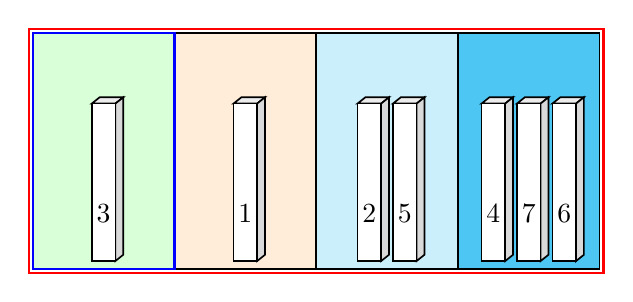
\begin{tikzpicture}[
			every node/.style={font=\normalsize},
			declare function={
				w=1.8;
				h=3;
				bw=0.3;
				bh=2.0;
				dx=0.1;
				dy=0.08;
				ybase=0.1;
			}
			]
			\fill[green!15] (0,0) rectangle ({w},{h});
			\fill[orange!15] ({w},0) rectangle ({2*w},{h});
			\fill[cyan!20] ({2*w},0) rectangle ({3*w},{h});
			\fill[cyan!70] ({3*w},0) rectangle ({4*w},{h});
			\draw[line width=0.6pt] (0,0) rectangle ({4*w},{h});
			\draw[line width=0.6pt] ({w},0) -- ({w},{h});
			\draw[line width=0.6pt] ({2*w},0) -- ({2*w},{h});
			\draw[line width=0.6pt] ({3*w},0) -- ({3*w},{h});
			\draw[draw=blue,line width=0.8pt] (0,0) rectangle ({w},{h});
			\draw[draw=red,line width=0.8pt] (-0.05,-0.05) rectangle ({4*w+0.05},{h+0.05});
			\def\drawbook#1#2{
				\draw[fill=gray!15,line width=0.6pt]
				(#1,{ybase+bh}) --
				({#1+dx},{ybase+bh+dy}) --
				({#1+bw+dx},{ybase+bh+dy}) --
				({#1+bw},{ybase+bh}) -- cycle;
				\draw[fill=gray!30,line width=0.6pt]
				({#1+bw},{ybase}) --
				({#1+bw+dx},{ybase+dy}) --
				({#1+bw+dx},{ybase+bh+dy}) --
				({#1+bw},{ybase+bh}) -- cycle;
				\draw[fill=white,line width=0.6pt]
				(#1,{ybase}) rectangle ({#1+bw},{ybase+bh});
				\node at ({#1+bw/2},{ybase+0.6}) {#2};
			}
			\drawbook{0.75}{3}
			\drawbook{2.55}{1}
			\drawbook{4.125}{2}
			\drawbook{4.575}{5}
			\drawbook{5.7}{4}
			\drawbook{6.15}{7}
			\drawbook{6.6}{6}
		\end{tikzpicture}
	\end{center}
	\par
	\shortans[oly]{806}
	\loigiai{
		Xét hình vẽ sau với mỗi ô vuông có đánh số $1$, $2$, $3$, $4$ lần lượt là các ngăn sách.
		\begin{center}
			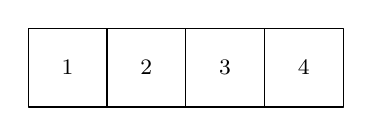
\begin{tikzpicture}[line cap=round, line join=round, >=stealth, font=\footnotesize, scale=1]
				\draw (0,0) rectangle (1,1) node[midway] {$1$} rectangle ++(1,-1) node[midway] {$2$} rectangle ++(1,1) node[midway] {$3$} rectangle ++(1,-1) node[midway] {$4$};
			\end{tikzpicture}
		\end{center}
		Bài toán yêu cầu xếp $7$ cuốn sách khác nhau vào $4$ ngăn phân biệt (có thứ tự), thứ tự sách trong mỗi ngăn cũng được tính. Ta thực hiện theo hai bước
		\begin{itemize}
			\item \textbf{Bước 1:} Xác định số lượng sách trong mỗi ngăn (bộ số lượng).
			\item \textbf{Bước 2:} Xếp $7$ cuốn sách cụ thể vào các vị trí đã định. Do $7$ cuốn sách khác nhau và các vị trí là phân biệt (ngăn $1$ vị trí $1$ khác ngăn $1$ vị trí $2$, và khác ngăn $2$ vị trí $1$\dots) nên với mọi cách chia số lượng, luôn có $7!$ cách xếp sách.
		\end{itemize}
		Phân tích các bộ số lượng sách $(n_1, n_2, n_3, n_4)$ thỏa mãn điều kiện
		\begin{itemize}
			\item Tổng số sách là $7$ nên $n_1+n_2+n_3+n_4=7$.
			\item Mỗi ngăn có ít nhất $1$ cuốn nên $n_i \ge 1$.
			\item Có ít nhất một ngăn $\ge 3$ cuốn.
		\end{itemize}
		Các bộ số lượng thỏa mãn (không kể thứ tự ngăn) là
		\begin{enumerate}
			\item Bộ $\{4; 1; 1; 1\}$ (có ngăn $4$ cuốn $\ge 3$).
			\item Bộ $\{3; 2; 1; 1\}$ (có ngăn $3$ cuốn $\ge 3$).
		\end{enumerate}
		
		\textbf{Tính số cách xếp cho từng trường hợp}
		\begin{itemize}
			\item \textbf{Trường hợp 1:} Bộ số lượng $\{4; 1; 1; 1\}$.\\
			Số cách phân chia số lượng vào $4$ ngăn là số hoán vị của $(4, 1, 1, 1)$. Vì có $3$ số $1$ giống nhau nên số cách là $\dfrac{4!}{3!} = 4$ cách.\\
			Số cách xếp sách là $4 \times 7!$.
			
			\item \textbf{Trường hợp 2:} Bộ số lượng $\{3; 2; 1; 1\}$.\\
			Số cách phân chia số lượng vào $4$ ngăn là số hoán vị của $(3, 2, 1, 1)$. Vì có $2$ số $1$ giống nhau nên số cách là $\dfrac{4!}{2!} = 12$ cách.\\
			Số cách xếp sách là $12 \times 7!$.
		\end{itemize}
		Tổng số cách xếp là
		\[T = (4 + 12) \times 7! = 16 \times 5040 = 80640 \text{ (cách)}.\]
		Giá trị cần tìm
		\[\dfrac{T}{100} = \dfrac{80640}{100} = 806{,}4 \approx 806.\]
	}
\end{ex}
%%%=============================%%%

%%%=============EX_22=============%%%
\begin{ex}%[1D2C1-6]
	\immini[thm]{Hỏi có tất cả bao nhiêu cách chọn ra $6$ số từ tập $\{1;2;3;4;5;6;7;8;9;10;11;12;13;14\}$ để xếp vào $6$ vị trí là $6$ điểm $A$, $B$, $C$, $M$, $N$, $P$ trong hình vẽ sao cho trên mỗi cạnh của tam giác $ABC$ luôn theo thứ tự lập thành một cấp số cộng có công sai nguyên?}{\begin{tikzpicture}[line cap=round, line join=round, >=stealth, font=\footnotesize, scale=.5]
			\def\r{0.5cm}
			\draw (0,0) coordinate (B) -- (60:6cm) coordinate (A) -- (0:6cm) coordinate (C) -- cycle;
			\filldraw[white] ($(B)!.5!(C)$) circle (\r) coordinate (M) ($(A)!.5!(C)$) circle (\r) coordinate (N) ($(B)!.5!(A)$) circle (\r) coordinate (P);
			\foreach \u in {A,B,C}{\filldraw[white] (\u) circle (\r);}
			\foreach \i in {A,B,C,M,N,P}{\draw (\i) circle (\r);
				\node at (\i) {$\i$};}
	\end{tikzpicture}}
	\par
	\shortans[oly]{312}
	\loigiai{
		Do các điểm $P$, $M$, $N$ lần lượt nằm trên các cạnh $AB$, $BC$, $CA$ và trên mỗi cạnh ba số theo thứ tự lập thành một cấp số cộng nên ta có
		\[
		\heva{
			A+B=2P,\\
			B+C=2M,\\
			C+A=2N.
		}
		\]
		Từ đó suy ra $A$, $B$, $C$ phải cùng chẵn hoặc cùng lẻ.\\
		Với mỗi bộ ba $(A;B;C)$ cùng chẵn hoặc cùng lẻ thì các số ở trung điểm được xác định duy nhất
		\[
		P=\dfrac{A+B}{2},\qquad
		M=\dfrac{B+C}{2},\qquad
		N=\dfrac{C+A}{2}.
		\]
		Muốn thỏa mãn yêu cầu của bài toán thì $P$, $M$, $N$ phải khác $A$, $B$, $C$. Điều này tương đương với việc trong bộ ba $(A;B;C)$ không được có số nào là trung bình cộng của hai số còn lại.\\
		Xét các số lẻ trong tập $\{1;3;5;7;9;11;13\}$.\\
		Số cách chọn ba số bất kỳ là $\mathrm{C}_7^3=35$.\\
		Các bộ ba lập thành cấp số cộng (không thỏa mãn) là
		\[
		(1;3;5),\ (3;5;7),\ (5;7;9),\ (7;9;11),\ (9;11;13),	(1;5;9),\ (3;7;11),\ (5;9;13),
		(1;7;13).
		\]
		Có tất cả $9$ bộ không thỏa mãn. \\
		Vậy số bộ ba số lẻ thỏa mãn là $35-9=26$.\\
		Xét các số chẵn trong tập $\{2;4;6;8;10;12;14\}$.\\
		Tương tự, ta cũng có $\mathrm{C}_7^3=35$
		bộ ba, trong đó các bộ lập thành cấp số cộng là
		\[
		(2;4;6),\ (4;6;8),\ (6;8;10),\ (8;10;12),\ (10;12;14),\ (2;6;10),\ (4;8;12),\ (6;10;14),\ (2;8;14).
		\]
		Cũng có $9$ bộ không thỏa mãn. \\
		Vậy số bộ ba số chẵn thỏa mãn là $35-9=26$.\\
		Suy ra tổng số bộ ba $(A;B;C)$ thỏa mãn điều kiện là $26+26=52$.\\
		Với mỗi bộ ba như vậy, khi xếp vào ba đỉnh $A$, $B$, $C$ của tam giác thì có $3!=6$ cách hoán vị. Ứng với mỗi cách xếp đó, ba số $P$, $M$, $N$ được xác định duy nhất bởi
		\[
		P=\dfrac{A+B}{2},\qquad
		M=\dfrac{B+C}{2},\qquad
		N=\dfrac{C+A}{2}.
		\]
		Vì vậy, tổng số cách xếp thỏa mãn đề bài là
		\[
		52\cdot 3! = 52\cdot 6 = 312.
		\]
		Vậy có tất cả $312$ cách xếp.
	}
\end{ex}
%%%=============================%%%
\Closesolutionfile{ans}

\newpage
\indapan{12}{ans/ansTN-Dung}
\indapan[TF]{2}{ans/ansTN-DungSai}
\indapan[SA]{6}{ans/ansTN-DienKhuyet}
%%%%%%%%%%%%%%
%%nhãn kết thúc đề (để đếm số trang tự động mỗi đề)
\label{B\thedeso}